\documentclass{article}

\usepackage[english]{babel}
\usepackage[utf8]{inputenc}
\usepackage{amsmath}
\usepackage{amsthm}
\usepackage{amssymb}
\usepackage{graphicx}
\usepackage{geometry}
\usepackage{float}
\newtheorem{theorem}{Theorem}
\newtheorem{definition}{Definition}
\newtheorem*{definition*}{Definition}

\title{A Time-Efficient Competitive Pok\'emon Team-Building Algorithm}
\author{Hugo Reijm, 4272692\\\\TU Delft}
\date{\today}
\selectlanguage{english}

\begin{document}
\maketitle

\newpage
\section*{Abstract}
The Pok\'emon video game franchise is based on players, also known as trainers, capturing and battling with fictitious creatures called Pok\'emon. Competitive Pok\'emon battling is a complicated business. Before even stepping into the arena, a trainer must design a competitively viable team of six Pok\'emon to battle with. This task is a difficult one because there are currently 721 species of Pok\'emon to construct a team from, and new Pok\'emon are revealed every year. The author therefore developed the Score-Based Pok\'emon Analysis algorithm, also known as SBPA, to aid users in easily and quickly designing new Pok\'emon teams.\\\\
The SBPA algorithm relies heavily on user interaction, and therefore requires the user to have already chosen at least one Pok\'emon to build his/her team around. The algorithm then analyzes the Pok\'emon the user has already chosen and returns a selection of Pok\'emon that would best further the development of the team. The user then chooses another team member, and the process is repeated until the user has developed his/her team. The SBPA algorithm analyzes the inputted team using three factors: Base Statistics, Typing, and the Popularity Factor. These three factors are then combined to determine the best potential team members per iteration.\\\\
The algorithm focuses not only on user interactivity, but also on time efficiency in order to provide valuable information to the user in a time frame that would be impossible to a technologically unaided trainer. As a cost for its speed and user-friendliness, SBPA is less accurate in determining the absolutely optimal team than certain other algorithms. However, when considering the target market of the algorithm, the author found these compromises worthwhile.

\newpage
\tableofcontents

\newpage
\section{Introduction}
Welcome to the Pok\'emon franchise! The Pok\'emon franchise is one that has existed since 1996, starting with the release of their first video games in Japan. Since then, it has become one of the world's most successful ``children's entertainment properties" in the world [1]. Among other merchandise, the Pok\'emon franchise specializes in the making of trading cards and related video games [16]. This thesis will focus on the latter.\\\\
The author attributes the astounding success the Pok\'emon video games have had to the incredible amount of variety and complexity present within the games' mechanics. So much potential for variation is present, that it has become difficult for competitive players to decide how to play the game. Therefore, the author developed a computer algorithm to mathematically analyze almost any situation a competitive player finds himself/herself in, and give advice in how to proceed. This algorithm has been named the Scored-Based Pok\'emon Analysis, or SBPA, algorithm.\\\\
This paper will give an in-depth look at the theory behind SBPA and its workings. However, before the algorithm can be fully comprehended, one must first understand the Pok\'emon games and more importantly the mechanics behind competitive Pok\'emon gameplay.

\section{An In-depth Look at Pok\'emon Mechanics}
The Pok\'emon video games are set in a world a little different from reality; this world is filled with creatures called Pok\'emon, short for ``Pocket Monster" [10,16]. What does a Pok\'emon look like? Almost anything. Just like there are many various animal species in the real world, so there are many different species of Pok\'emon in the Pok\'emon world. In the case of Pok\'emon, there are currently 721 different usable species of Pok\'emon, and more are revealed every year [10]. What makes things even more complicated is that several Pok\'emon species have multiple forms that they can take on in and out of battle. An example of such a Pok\'emon species is Species \#386, also known as Deoxys. An individual Deoxys can take on one of four forms, shown below:
\begin{figure}[H]
\begin{minipage}{.25\textwidth}
	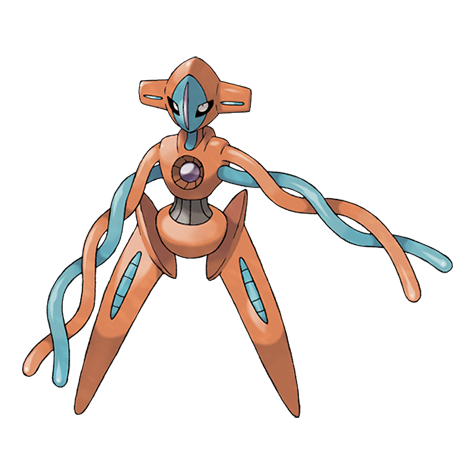
\includegraphics[width=\textwidth]{386_f1.png}
\end{minipage}%
\begin{minipage}{.25\textwidth}
	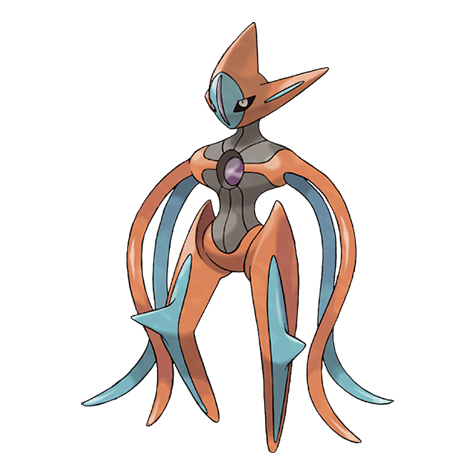
\includegraphics[width=\textwidth]{386_f2.png}
\end{minipage}%
\begin{minipage}{.25\textwidth}
	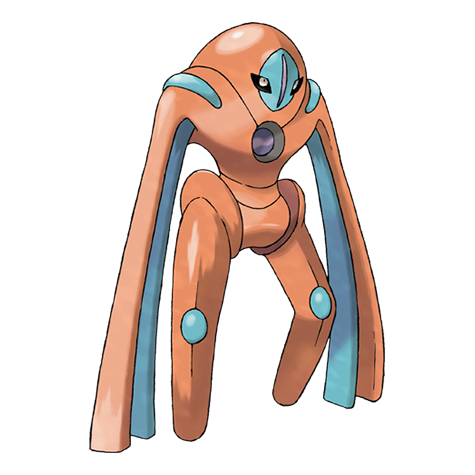
\includegraphics[width=\textwidth]{386_f3.png}
\end{minipage}%
\begin{minipage}{.25\textwidth}
	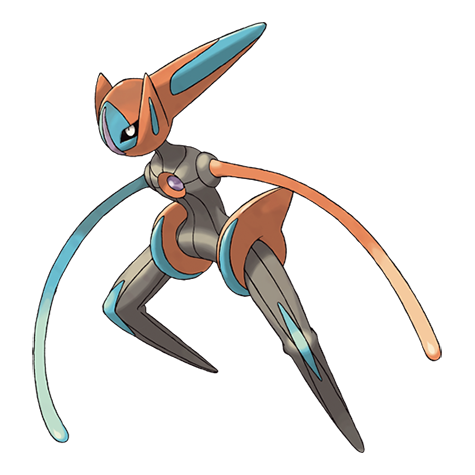
\includegraphics[width=\textwidth]{386_f4.png}
\end{minipage}
\centering
\caption{Image credits goes to the Pok\'emon Company International [6]}
\end{figure}
Although each form can provide certain benefits to Deoxys that the other forms can not, the forms are still considered to be of the same species [6]. For the sake of simplicity, the author has for the most part ignored these forms in this thesis; however he has taken these into account in SBPA.\\\\
The Pok\'emon shown in Figure~\ref{fluffypic} will be used as an example from now on:
\begin{figure}[H]
	
\includegraphics[width=0.30\textwidth]{fluffy.png}
	\centering
	\caption{Image credit goes to the Pok\'emon Company International [27]}\label{fluffypic}
\end{figure}
This is a Pok\'emon nicknamed ``Fluffy". He is an individual of Pok\'emon species~\#263, named Zigzagoon. Zigzagoons are about the size of a small dog [27].\\\\
Players of the Pok\'emon games can catch and train Pok\'emon like Fluffy in order to battle other players and their Pok\'emon. Therefore, players are also referred to as trainers. This concept is what the Pok\'emon video games center around: the player becoming stronger by catching and battling other Pok\'emon [16].\\\\
Over the years, players from all over the world have started to battle each other in this way. They have strategized and trained their Pok\'emon to peak performance in order to become the very best. This is called competitive Pok\'emon battling. This competition has its climax every year during the Pok\'emon VG World Championships, which was held last year in Boston [20].
The workings of one of these competitive matches will be briefly discussed in the following section.

\subsection{A Typical Pok\'emon Battle}\label{BattleFormatSection}
Before a trainer can battle another trainer, he/she must construct a team. 
\begin{definition}
	A \textbf{Team} is a collection of six individual Pok\'emon.
\end{definition}
Teams contain the Pok\'emon necessary for a trainer to play out his/her battle strategy. Once a trainer has engaged in battle, he/she may only battle with the Pok\'emon in the one team he/she chose to take into battle [14,17].\\\\
Constructing a team requires a considerable amount of thought. First off, the one constructing a team must decide which tiers he/she wishes to select his/her Pok\'emon team members from.
\begin{definition}\label{tierdef}
	Not all Pok\'emon are made equal; they are ranked according to their power and potential into sets called \textbf{Tiers}. In general, a tier is ranked based on the average power and potential of the Pok\'emon within this tier: the higher the tier's rank, the more powerful the Pok\'emon within the tier generally are $[7]$.
\end{definition} 
Some formats of battle only allow for Pok\'emon from certain tiers to be used in a team. This is done in order to establish not only fairness in battle, but also allowing for diversity in teams [9]. If a trainer wishes to participate in a certain battle format, he/she must know which Pok\'emon are allowed to be used in a team and which are not. Generally, a battle format's name is the same as the highest ranked tier from which members are still allowed to participate in battle. All Pok\'emon from lower-ranked tiers may always participate in these particular battle formats. For the battle formats that the SBPA algorithm focuses on, this is always the case.\\\\
SBPA focuses on seven different battle formats in order to give the user a significant amount of choice. The seven different formats are:
\begin{itemize}
	\item \textbf{Anything Goes}, abbreviated here as AG, which allows all 721 Pok\'emon species to battle, a total of 817 different Pok\'emon if including Pok\'emon forms [2]
	\item \textbf{Uber}, which also allows all 721 Pok\'emon species to battle. However, it forbids a certain form of a certain Pok\'emon species to battle, resulting in a total of 816 different Pok\'emon if including Pok\'emon forms [25]
	\item \textbf{Battle Spot Singles}, abbreviated here as BS, which is the official battle format in the Pok\'emon games and allows 690 Pok\'emon species to battle, a total of 753 different Pok\'emon if including Pok\'emon forms [4]
	\item \textbf{Over Used}, abbreviated OU, which allows 701 Pok\'emon species to battle, a total of 760 different Pok\'emon if including Pok\'emon forms [13]
	\item \textbf{Under Used}, abbreviated UU, which allows 656 Pok\'emon species to battle, a total of 687 different Pok\'emon if including Pok\'emon forms [26]
	\item \textbf{Rarely Used}, abbreviated RU, which allows 584 Pok\'emon species to battle, a total of 602 different Pok\'emon if including Pok\'emon forms [21]
	\item \textbf{Never Used}, abbreviated NU, which allows 527 Pok\'emon species to battle, a total of 539 different Pok\'emon if including Pok\'emon forms [12]
\end{itemize}
The author chose to focus on these particular formats due to experience that told him that these were the most common.
The graph below visualizes the number of Pok\'emon species and forms allowed in the seven formats described above:
\begin{figure}[H]
	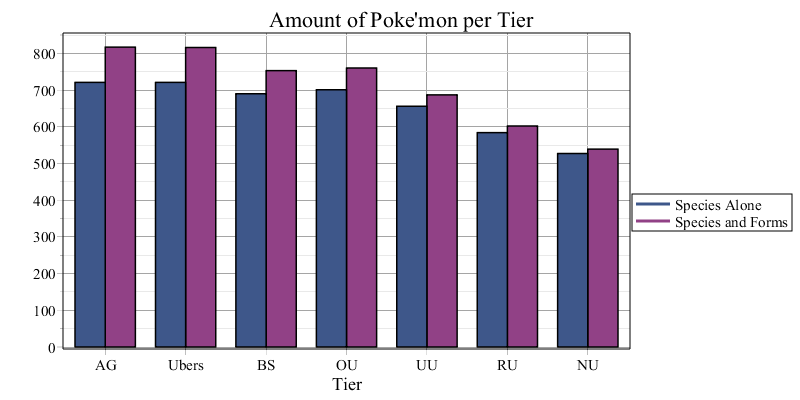
\includegraphics[width=\textwidth]{TierAmount.png}
	\centering
	\caption{}\label{TierAmountGraph}
\end{figure}
Obviously, should a trainer want to construct a team for a battle format that allows a large set of Pok\'emon, the SBPA algorithm will require more time to run to completion than for a battle format that allows a smaller set of Pok\'emon; more data to analyze requires more time to do so. This fact becomes apparent in later analysis.\\\\
Furthermore, most battle formats enact certain clauses. A clause that is very pertinent to Pok\'emon team building itself is the Species Clause.
\begin{definition}\label{SpeciesClause}
	The Species Clause requires any competitive trainer to use six Pok\'emon of different species in his/her team [9].
\end{definition}
In other words, a trainer may only use our example Pok\'emon Fluffy once in a team, and no other individual of Fluffy's species may be present in that same team. Out of all the battle formats that SBPA focuses on, only the Anything Goes format does not enact this clause [2]. However, the algorithm still assumes that all of the formats do enact it in order to generate teams with various team members and to preserve a certain uniformity in the coding.\\\\
The Species Clause provides a way of estimating the total number of Pok\'emon teams that could be built. Assuming that any of the 721 species could be used in the construction of a team while ignoring different Pok\'emon forms, a quick calculation reveals the maximum number of groupings of six different Pok\'emon species one could put together:
\begin{equation*}
	\left({721 \above 0pt 6}\right)=1.91082439565304\text{ x }10^{14}
\end{equation*}
Roughly 200 trillion different groups of six different Pok\'emon species can be made. Note that this is not the total number of Pok\'emon teams that can be made; the maximum number of actual teams is far greater. The Pok\'emon Company designed individual Pok\'emon to be moderately modifiable. A player can to a certain extent modify every Pok\'emon in his/her team in order to maximize the team's win-lose ratio. This can be done in several ways, which this thesis will not get into. However, it is clear that individuals from a Pok\'emon species can be widely differing from each other, and thereby significantly increasing the number of Pok\'emon teams that could be made [9]. This is the reason why the SBPA algorithm is more complex than just brute-force calculating which team would be best in a certain situation: the runtime to compute this would be far too impractical for such an approach.\\\\
For simplicity, SBPA does not focus on every possible Pok\'emon individual, but rather removes these individualities and analyzes the species as a whole. Remember that a Pok\'emon is moderately modifiable. This would imply that Pok\'emon species have a default setting, which happens to be the same for all individuals of that Pok\'emon species [18]. Therefore, the algorithm focuses on these default settings, thereby still providing viable team-building advice while reducing runtime significantly.\\\\
Once a trainer has constructed a team that is allowed by the battle format he/she wishes to participate in, the trainer is automatically matched with an opponent through a computer system. Both trainers start by viewing a basic overview of their opponent's team. In this Team Preview, nothing is revealed about the opponent's team except which Pok\'emon it contains. Based on this, each player privately decides in which order to send his/her Pok\'emon into battle. Once both players have made their decisions, the battle begins [11].\\\\
A Pok\'emon battle is a turn-based system. Each turn begins with both players privately selecting their preferred actions for that turn. Once both players have decided what they will do for that turn, the results of the players' decisions is played out and a new turn begins. This cycle is repeated until one player has no more usable Pok\'emon to battle with, a situation which usually results from all the player's Pok\'emon being ``knocked out" by the opponent's Pok\'emon. When this happens, the player with no usable Pok\'emon loses the match [17]. In the rare case that both players lose their last Pok\'emon simutaneously, the victor is decided by who hit last [9].\\\\
This is a basic overview of a competitive Pok\'emon battle. Many variations in battle style exist, but all can be boiled down to this system.\\\\
The quality of a Pok\'emon team could therefore be described as follows. The human element in this case is removed from the definition for simplicity's sake:
\begin{definition}\label{QualityDef}
	Say that a trainer uses team $t$ in $N$ battles, from which he/she wins $n$ times. Then the quality of team $t$ is $n/N$, where $n\le N$ and $N>\!>1$ 
\end{definition}
Therefore, for a team to have a high quality, the trainer must think of all the factors involved in building a team and optimize them. This thesis will analyze a certain set of these factors in a bottom-up fashion, relying on the philosophy that one can not fully understand the whole without understanding all the parts. Therefore, the next few sections describe the mechanics of individual Pok\'emon, because one can not fully understand a team without understanding all the intricacies of a single Pok\'emon.

\subsection{Individual Pok\'emon Mechanics}
Pok\'emon, even at an abstract level, are complex creatures with many various characteristics. As per earlier, observe Fluffy. He may look simple, but a further analysis reveals the following:
\begin{figure}[H]
	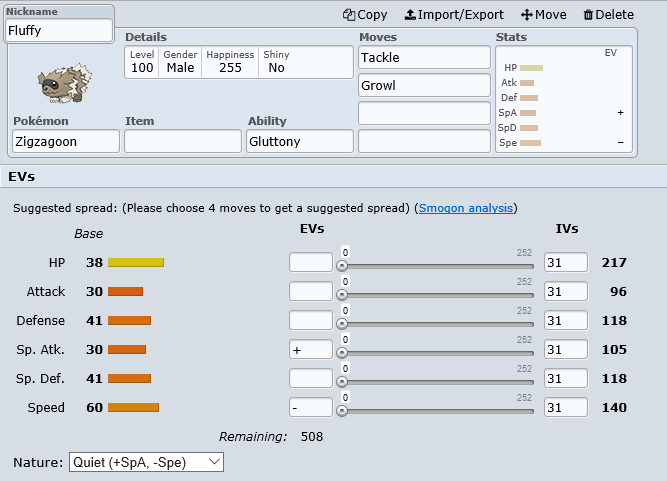
\includegraphics[width=0.9\textwidth]{fluffyfile.png}
	\centering
	\caption{Screen shot from Fluffy's custom-made Pok\'emon Showdown! file, sponsored by Smogon University [18]}\label{FluffyFile}
\end{figure}
This is Fluffy expressed in numbers and figures; a rather large set of mathematical data. Due to time constraints in the developmental phase, the SBPA algorithm does not take into account many of the factors present here. Therefore, SBPA is an algorithm that merely gives advice; it can not calculate ever single situation to result in a perfect optimum. However, SBPA can still give viable advice by using two important factors found in every Pok\'emon: Base Statistics and Typing.

\subsubsection{Base Statistics}
Taking another look at Fluffy and his file, observe the following section:\\
\begin{figure}[H]
	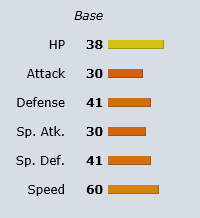
\includegraphics[width=0.4\textwidth]{fluffystats.png}
	\centering
	\caption{Photo credit goes to Pok\'emon Showdown!, sponsored by Smogon University [18]}
\end{figure}
These are Fluffy's Base Statistics. 
\begin{definition}
	\textbf{Base Statistics}, also know as ``Base Stats", are a set of six integers that determine how well a Pok\'emon can fill a certain role in a team.
\end{definition}
For example, if a Pok\'emon team requires a new member that is incredibly fast, then the trainer will have to search for a Pok\'emon with a very high Speed Stat. Fluffy's Base Stats are not very high when compared to other Pok\'emon, which accounts for the fact that Fluffy's species does not see much competitive play.\\\\
The following definitions shed light on what each Base Stat stands for:
\begin{itemize}
	\item The \textbf{HP} Base Stat stands for the Hit Points that a Pok\'emon has. Very basically, Hit Points determines how large of an attack the defending Pok\'emon can survive [23].
	\item The \textbf{Attack} Base Stat stands for the physical power a Pok\'emon possesses. If a Pok\'emon were to use a physically attacking move, such as throwing a punch, then the power of that move would be determined by this Base Stat [15,23]. 
	\item The \textbf{Defense} Base Stat stands for how well a Pok\'emon can defend itself from physical moves~[23]. 
	\item The \textbf{Sp.Atk.} Base Stat, an abbreviation for ``Special Attack", stands for the Special power a Pok\'emon possess. The word ``Special" refers to any move that doesn't include direct physical contact between the attacking and defending Pok\'emon. Examples of such moves are ``Thunderbolt", ``Shadow Ball", and ``Telekinesis" [22,23].
	\item The \textbf{Sp.Def.} Base Stat, an abbreviation for ``Special Defense", stands for how well a Pok\'emon can defend itself from Special moves [23].
	\item The \textbf{Speed} Base Stat stands for how fast a Pok\'emon is. In a battle, the Speed Base Stat determines which Pok\'emon moves first in a turn [23].
\end{itemize}
A trainer that is building a Pok\'emon team must keep track of how the Base Stats of the team members interact with each other. Perhaps the trainer wants to make a team that is more aggressive than most teams. That would entail that he/she needs to put more focus on the overall Attack, Special Attack, and Speed of his/her team. Perhaps he/she wishes to make a slower, defensive team. Then the overall HP, Defense, and Special Defense of the team are of more importance.\\\\
For simplicity's sake, assume that Base Stats are species-dependent characteristics; that is to say: every individual of a Pok\'emon species has the same Base Stats. Technically, Base Stats can change from individual to individual due to modifiers, but analyzing these would be too complicated and time-consuming [3]. The SBPA algorithm assumes that Base Stats are species-dependent, thus resulting in the algorithm not looking at every possible individual of every possible Pok\'emon species, but merely looking a species as a whole. As discussed before, this makes the algorithm much more time-efficient.

\subsubsection{Typing}
Another species-dependent characteristic is Typing. Every species can have up to two Types, which classify what that Pok\'emon species is. For example, recall that Fluffy is an individual of Pok\'emon species \#263. All individuals of species \#263 have only one Type: the ``Normal" Type [27]. This attribute is not shown in Figure \ref{FluffyFile}.\\\\
There are 18 Types in total: Bug, Dark, Dragon, Electric, Fairy, Fighting, Fire, Flying, Ghost, Grass, Ground, Ice, Normal, Poison, Psychic, Rock, Steel, and Water. These Types interact with each other in a complex game similar to Rock-Paper-Scissors [24]. The situation is more complicated, however, because of Weaknesses, Resistances, and Immunities. The basic definitions are given below:
\begin{definition*}
	A Type's \textbf{Weaknesses} are a set of Types. If a Pok\'emon were to be attacked by an opposing Pok\'emon, where the Typing of the attacking Pok\'emon happened to be in the set of Weaknesses of the defending Pok\'emon, then the attacking Pok\'emon would do $m$-times more damage than normal. Usually, $m$ is equal to 2. This would also be known as a Super Effective attack $[5,24]$.
\end{definition*}
\begin{definition*}
	A Type's \textbf{Resistances} are a set of Types. If a Pok\'emon were to be attacked by an opposing Pok\'emon, where the Typing of the attacking Pok\'emon happened to be in the set of Resistances of the defending Pok\'emon, then the attacking Pok\'emon would do $n$-times less damage than normal. Usually, $n$ is equal to 2. This would also be known as a Not Very Effective attack~$[5,24]$.
\end{definition*}
\begin{definition*}
	A Type's \textbf{Immunities} are a set of Types. If a Pok\'emon were to be attacked by an opposing Pok\'emon, where the Typing of the attacking Pok\'emon happened to be in the set of Immunities of the defending Pok\'emon, then the attacking Pok\'emon would do no damage at all. This would also be known as a Not Effective attack $[5,24]$.
\end{definition*}
The following chart shows the weaknesses (green squares), resistances (red squares), and immunities (dark grey squares) of each Pok\'emon Type, whereby a Pok\'emon with a Type in the column on the right is attacking a Pok\'emon with a Type in the row on top.
\begin{figure}[H]
	\includegraphics[width=0.9\textwidth]{TypeChart.png}
	\centering
	\caption{The Type Chart found in The Pok\'emon Database [19]}
\end{figure}
To further complicate matters, remember that every Pok\'emon species can have a minimum of one, maximum of two Types. Should a Pok\'emon have two Types, then those Types could cancel out each other's weaknesses with their resistances and vice versa. However, these Type could also interfere constructively, resulting in a species with a double weakness or a double resistance to a certain Type [24].\\\\
Therefore, in competitive Pok\'emon battling, a trainer must try to form a team where the members
\begin{itemize}
	\item balance out each other's weaknesses with their resistances.
	\item have enough variety amongst themselves so that they can deal with as many different Pok\'emon and their associated Types as possible.
\end{itemize}
The Pok\'emon gameplay mechanics discussed above are the predominant characteristics of individual Pok\'emon that the SBPA algorithm will take into account. As stated previously, this algorithm is by no means perfect; it merely gives advice for the situation at hand. It ignores many gameplay mechanics that are far too complex to program into the algorithm in the allotted time for this project. However, as one shall see below, the algorithm still is able to give valuable information to the user in a time-efficient manner.

\section{The Mechanics Behind the Algorithm}
Now that the necessary background information has been established and documented, the SBPA algorithm can be described in detail. SBPA is a user interactive, iteration-based computer algorithm written in Java. The author chose not to use Matlab or Maple as the main programming platform because Java is not only more convenient to share with other people, but also because writing the algorithm in Java deemed more useful to the author. This section will describe the mathematical theory behind SBPA; software details will be ignored unless they have pertinence in relation to the mathematics.\\\\
At the very beginning, the algorithm requires the user to input which tiers the user wants to use, the style of team the user wants to make (whether it be defensive, balanced, or aggressive), and at least one Pok\'emon that the user wants to build a team around. The program then has all the necessary information for it to start its first iteration. Every iteration follows the same procedure:
\begin{enumerate}
	\item Gather the necessary information from the partial team that the user has already put into the algorithm. The program then uses the Species Clause (Definition \ref{SpeciesClause}) to remove any potential violators from the list of Pok\'emon species that the algorithm needs to run through.
	\item For every Pok\'emon in the list determined in the previous step, apply a series of self-designed scoring systems and give an overall score based on these systems.
	\item Sort the list from Step 1 in descending order based on the scores found in the previous step.
	\item Display the first $K$ results from the sorted list and wait until the user has chosen a Pok\'emon for his/her team based on the displayed suggestions or his/her own decision.
\end{enumerate}
In other words, SBPA takes into account the partial team that the user already has and suggests the best addition to that team based on a self-designed scoring system. As one can see, SBPA was designed to be very input-driven; it relies heavily on the input of the user to complete an iteration. Once it has scored which Pok\'emon would be the best addition to the user's team, it waits for further input. This process repeats until the user has assembled a team of six Pok\'emon, at which point the algorithm no longer searches for more potential team members. Because the user starts by inputting the first Pok\'emon, the algorithm requires five iterations to help the user generate an entire team.\\\\
Attention must be paid to the fact that this methodology of constructing a team could be substituted for another. Notice that the SBPA algorithm does not guarantee the user an absolutely optimal team; other methodologies could ensure this. However, the author chose to use this methodology for a few reasons. First off, he wanted to construct a time efficient algorithm so that runtime would not become a hindrance when users construct a team using his program. But more importantly, he wanted to preserve user interactivity. Even if the author were to use optimization techniques that efficiently found the absolutely optimal team, they would by definition ignore the user's personality, style, and preferences. The author has the following philosophy when concerning himself with trainers and their teams: half the credit of a victory goes to the trainer, and the other half goes to the trainer's team. Together they form one entity. The trainer must therefore know everything about his/her team and play an active role its development. Solving for an absolutely optimal team through perhaps the Simplex algorithm would remove this interactivity from the team building process. The SBPA algorithm could be expanded to include such an optimization technique in the future, but this would only be used to provide more information to the user so that he/she can make the ultimate decision. For all of these arguments, the author chose the methodology described in this thesis.\\\\
The accuracy and efficiency of SBPA depend on what scoring systems have been implemented in its coding. However, there is no absolute scoring system for deciding whether a Pok\'emon is a ``good" or ``bad" candidate for a team. Therefore, the scoring system can not be based on an absolute score, but must be based on a relative one, comparing Pok\'emon to each other to find a solution. The overal scoring system takes three factors into account: a Pok\'emon's Base Stats, a Pok\'emon's Typing, and a Pok\'emon's Popularity Factor. These scoring factors build upon each other as depicted in the diagram below:
\begin{figure}[H]
	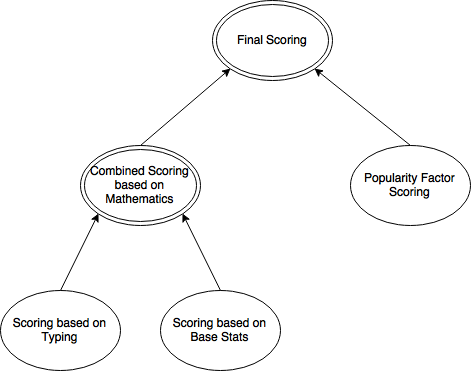
\includegraphics[width=0.7\textwidth]{ScoringDiagram.png}
	\centering
	\caption{Diagram Showing the Composition of the Scoring System}\label{ScoringComposition}
\end{figure}
The composition and combination of the scoring factors is explained in the sections below.
\subsection{Scoring Based on Base Stats}\label{scoringBaseStats}
As discussed earlier, the Base Stats of a Pok\'emon determine how well that Pok\'emon can fulfill certain roles in a team. Therefore, a logical approach to determining a score for a Pok\'emon is to analyze how well it fills the roles that the partial team of the user still needs to fill.\\\\
The algorithm does this by using the following equation:
\begin{equation}\label{statsScoreEqn}
	S(t,P)_{Stats}=(\textbf{A}(t\cup P)-\textbf{A}(T_{max}))\bullet\textbf{M}_{Stats}
\end{equation}
Here, $S(t,P)_{Stats}$ stands for the score given to Pok\'emon $P$, relative to its Base Stats and the user's already partially constructed team $t$. The real vector $\textbf{A}(t\cup P)$ contains the averages of the Base Stats of partial team $t$ with the addition of Pok\'emon $P$, where:
\begin{itemize}
	\item $\textbf{A}(t\cup P)_1$ is the average HP Base Stat of $P$ and all Pok\'emon in $t$
	\item $\textbf{A}(t\cup P)_2$ is the average Attack Base Stat of $P$ and all Pok\'emon in $t$
	\item $\textbf{A}(t\cup P)_3$ is the average Defense Base Stat of $P$ and all Pok\'emon in $t$
	\item $\textbf{A}(t\cup P)_4$ is the average Special Attack Base Stat of $P$ and all Pok\'emon in $t$
	\item $\textbf{A}(t\cup P)_5$ is the average Special Defense Base Stat of $P$ and all Pok\'emon in $t$
	\item $\textbf{A}(t\cup P)_6$ is the average Speed Base Stat of $P$ and all Pok\'emon in $t$
\end{itemize}
The vector $\textbf{A}(T_{max})$ is constructed in a similar way; however it contains the average Base Stats of the Pok\'emon in the highest ranked tier $T_{max}$ allowed in the battle format that the user is working with.\\\\
Vector $\textbf{M}_{Stats}$ is also constructed in much the same way as $\textbf{A}(t\cup P)$. However, rather than each of $\textbf{M}_{Stats}$'s elements representing the average of a Base Stat, they instead stand for a Base Stats' bias, dependent on the user's preference of team style. Perhaps the user wants to construct a team that, for example, is more aggressive when compared to other teams. In that case, Pok\'emon with high Attack, Special Attack, and Speed Base Stats are of more importance than Pok\'emon with high HP, Defense, and Special Defense Stats. The bias vector $\textbf{M}_{Stats}$ was therefore introduced in order to give the user the ability to choose which Base Stats on average matter more for the user's team. The algorithm gives three options in team style: Defensive, Balanced, and Aggressive. The bias vector is then chosen as follows:
\begin{itemize}
	\item $\textbf{M}_{Stats}=[\frac{9}{30},\frac{1}{30},\frac{9}{30},\frac{1}{30},\frac{9}{30},\frac{1}{30}]^T$ when the user builds a Defensive team
	\item $\textbf{M}_{Stats}=[\frac{1}{6},\frac{1}{6},\frac{1}{6},\frac{1}{6},\frac{1}{6},\frac{1}{6}]^T$ when the user builds a Balanced team
	\item $\textbf{M}_{Stats}=[\frac{1}{30},\frac{9}{30},\frac{1}{30},\frac{9}{30},\frac{1}{30},\frac{9}{30}]^T$ when the user builds an Aggressive team
\end{itemize}
The exact values of these vectors are based on the author's intuition and choice to generate a noticeable difference between team styles. However, the values have been set in such a way that the sum of the elements in $\textbf{M}_{Stats}$ is always equal to 1. That way, $S(t,P)_{Stats}$ is the weighted sum of the elements of $(\textbf{A}(t\cup P)-\textbf{A}(T_{max}))$, which therefore takes into account all the given data while still awarding higher importance to certain Base Stats according to the user's team style selection.\\\\
In theory (and also of course in practice), Equation \ref{statsScoreEqn} first scores Pok\'emon $P$ on the impact it would have when added to partial team $t$, relative to the average Base Stats of tier $T_{max}$. This score is then combined with the previously discussed bias $\textbf{M}_{Stats}$ into a dot product to result in a final scalar score. The dot product operator was chosen for two reasons. First of all, the dot product is a simplistic operation that is easy to understand and relatively time-efficient. But more importantly, the dot product allows the scoring to take into account the influence of every Base Stat of $P$ and not just the largest or most important for example. Thereby, SBPA can completely and throughly evaluate $P$ based on its Base Stats, yet still do this in an efficient manner.

\subsection{Scoring Based on Typing}
The SBPA algorithm also scores a Pok\'emon based on its Typing. Keeping track of a team's overall Typing is important so that any glaring weaknesses or excessive investment in a certain resistance can be avoided. Therefore, Pok\'emon are scored based on the weaknesses, resistances, and immunities that the user's partial team already has.\\\\
In this case, the scoring uses the equation below, which again is based on vectors and dot products:
\begin{equation}\label{TypeScoreEqn}
	S(t,P)_{Type}=(\textbf{T}(t\cup P)-\textbf{T}(t))\bullet\textbf{M}_{Type}
\end{equation}
In this case, $S(t,P)_{Type}$ is the score given to a Pok\'emon $P$ relative to its Typing.\\\\
Vector $\textbf{T}(t)$ is a integer vector that described how well partial team $t$ handles opposing Pok\'emon of a certain Type. The vector needs to monitor how well $t$ interacts with all Types; since there are 19 Types (18 Pok\'emon Types and one added NULL Type for computational simplicity), $\textbf{T}(t)$ is 19 elements long. Every iteration, the elements of $\textbf{T}(t)$ are reset to zero. Every element $\textbf{T}(t)_i$ is then calculated as described below.\\\\
For every Pok\'emon $j$ in partial team $t$:
\begin{itemize}
	\item $\textbf{T}(t)_i=\textbf{T}(t)_i-1$ if Pok\'emon $j$ in $t$ is weak to Type $i$
	\item $\textbf{T}(t)_i=\textbf{T}(t)_i+1$ if Pok\'emon $j$ in $t$ is resistant to Type $i$
	\item $\textbf{T}(t)_i=\textbf{T}(t)_i+2$ if Pok\'emon $j$ in $t$ is immune to Type $i$
\end{itemize}
The vector $\textbf{T}(t\cup P)$ is calculated much in the same way, except for the fact that it monitors how well $t$ would handle certain Types if Pok\'emon $P$ were to be added to it.\\\\
The bias vector $\textbf{M}_{Type}$ is present in this equation to once again dictate what is more important and what is less important. At the moment, the Types are dictated as being equivalently important for simplicity's sake, but a possible update to the program could be the implementation of a bias vector $\textbf{M}_{Type}$ that changes as the user's team grows. More research in this field is necessary to discover how such a bias vector could be computed.\\\\
The Equations \ref{statsScoreEqn} and \ref{TypeScoreEqn} are structured in a similar way, and thus the mathematical theories behind both equations are almost identical. Just as in Equation \ref{statsScoreEqn}, $S(t,P)_{Type}$ is based on the Typing benefits that Pok\'emon $P$ could add to partial team $t$. Once that has been computed, a dot product is taken with the bias vector $\textbf{M}_{Type}$ in order to efficiently combine all elements of $(\textbf{T}(t\cup P)-\textbf{T}(t))$ and $\textbf{M}_{Type}$ into a scalar value.

\subsection{Scoring Based on Popularity Factor}
As explained before, a Pok\'emon isn't defined merely by its Base Stats and Typing. Unfortunately, most other characteristics are time-consuming to program and could not be included in the mathematics of the SBPA algorithm in the allotted time. However, a method was devised to still take a shadow of these characteristics into account: the Popularity Factor $S(t,P)_{Pop}$.\\\\
The Popularity Factor is based on the past experiences of other players. Since the Pok\'emon franchise is one of the most successful of all time, thousands of people battle every day in order to improve their skills and become the very best that they can be [16]. With that many players, certain patterns start to evolve over time, centering around successful strategies. One could compare the world-wide group of competitive Pok\'emon trainers as an immense, learning computer program; its purpose being to seek out new battle strategies while preserving those of high quality (A team's quality is defined in Definition \ref{QualityDef}). It would be foolish to not use all the successful strategies that have been found thus far.\\\\
The Popularity Factor is not a mathematics-based construct; rather, it is based on collecting as many teams as possible and storing them in such a way that they can later be requested and used in a time-efficient manner. Therefore, the author constructed a integer-valued matrix~$\textbf{P}_{T_f}$ for battle format $f$'s set $T_f$ of allowed Pok\'emon (For a reminder of what battle formats are, read Section \ref{BattleFormatSection}, starting at Definition \ref{tierdef}). In $\textbf{P}_{T_f}$, every Pok\'emon allowed by format~$f$ has its own separate column and its own separate row. Note that the matrix for the format that allows $k$ Pok\'emon to battle has $k$ columns and $k$ rows, resulting in $k^2$ different elements. This is quite a large matrix and thus quite a large portion of data. However, doing so allows for data requests to be completed simply and quickly, as will be shown later on.\\\\
At first, all the elements in these matrices are zero. Populating these matrices with useful data is done as follows. Let's say the author finds a Pok\'emon team $t$, allowed by set $T_f$ in battle format~$f$, that he wishes to use as data for SBPA. He already has written a program to import any team he wishes into the algorithm. The program scans through $t$ and imports only the names of the Pok\'emon species present in the team; all other characteristics are not included in order to decrease the algorithm's runtime as much as possible. The program then finds the rows and columns in $\textbf{P}_{T_f}$ corresponding to each of the members of $t$, and groups them into sets $R_t$ and $C_t$ respectively. The matrix $\textbf{P}_{T_f}$ is then updated as follows:
\begin{equation*}
	\textbf{P}_{T_f,r,c}=\textbf{P}_{T_f,r,c}+1\text{, }r\in R_t\text{ and }c\in C_t
\end{equation*}
In this way, $\textbf{P}_{T_f}$ is built to register patterns between Pok\'emon species in teams. The larger an element of $\textbf{P}_{T_f}$, the more people use the two Pok\'emon corresponding to that element in a team, and thus the more likely that the two corresponding Pok\'emon work well together. What is more, this method does not depend on Pok\'emon Base Stats or Typing, resulting in a simple method capable of finding effective Pok\'emon team combinations that would otherwise go unnoticed in the analysis of Base Stats and Typing.\\\\
Understanding all this, the Popularity Factor $S(t,P)_{Pop}$ is simple to express for Pok\'emon $P$ and partial team $t$ allowed in set $T_f$ of battle format $f$:
\begin{equation}\label{popScoreEqn}
	S(t,P)_{Pop}=\sum_{s\in t}\textbf{P}_{T_f,s,P}
\end{equation}
In other words, $S(t,P)_{Pop}$ is simply a measure to see how many times Pok\'emon $P$ and a member of partial team $t$ have been members of the same team in the past.

\subsection{Combining Scoring factors}
Combining Equations \ref{statsScoreEqn}, \ref{TypeScoreEqn}, and \ref{popScoreEqn} takes some thought. As stated earlier, there is no absolute measure for deciding whether Pok\'emon $P$ is a ``good" or ``bad" candidate for partial team $t$. Rather, the final score given to $P$ should be a relative one, comparing $P$'s score to that of all the other candidates.\\\\
The author decided to combine the scoring systems in such a way as to meet the following criteria:
\begin{enumerate}
	\item Results for Equation \ref{TypeScoreEqn} should be about 1.4 times as important as results from Equation \ref{statsScoreEqn}. This observation comes from Jenty Heijstek, a competitive trainer who came in fourth place during the Dutch National Video Game Tournament in 2013 [8]. Furthermore, Equations \ref{statsScoreEqn} and \ref{TypeScoreEqn} should be combined into one scoring system based on mathematics alone, with Equation~\ref{popScoreEqn} added later (See Figure \ref{ScoringComposition}). In this way, compartmentalization occurs, which organizes the scoring systems and allows for the relative ease of implementing new scoring systems to the algorithm in possible later updates.
	\item The importance of Equation \ref{popScoreEqn} should decrease as more Pok\'emon are added to the user's team, while at the same time the importance of the scoring sytem based on Equations \ref{statsScoreEqn} and~\ref{TypeScoreEqn} should increase. This is because as a team nears completion, all imperfections and glaring flaws still present in the team need to be compensated for, which is much more easily done when focusing on Base Stats and Typing than when focusing on the Popularity Factor. 
\end{enumerate}

\subsubsection{Criterion 1}
The first part of Criterion 1 can easily be met by performing the following scaling transformations on $S(t,P)_{Stats}$ and $S(t,P)_{Type}$:
\begin{eqnarray*}
	S'(t,P)_{Stats}=(S(t,P)_{Stats}-\min_P(S(t,P)_{Stats}))*\cfrac{10}{\max_P(S(t,P)_{Stats})-\min_P(S(t,P)_{Stats})}\\
	S'(t,P)_{Type}=(S(t,P)_{Type}-\min_P(S(t,P)_{Type}))*\cfrac{10}{\max_P(S(t,P)_{Type})-\min_P(S(t,P)_{Type})}
\end{eqnarray*}
Through this transformation, both $S(t,P)_{Stats}$ and $S(t,P)_{Type}$ are changed to always have a range equal to the interval [0,10] in $\mathbb{Z}$, thereby removing any bias that could result from the two scoring systems having different ranges. Unfortunately, these transformations needs to be performed every iteration of the algorithm since $\max_P(S(t,P)_{Stats})$, $\min_P(S(t,P)_{Stats})$, $\max_P(S(t,P)_{Type})$, and $\min_P(S(t,P)_{Type})$ take on different values for every iteration. However, a computer can easily perform such transformations, so thankfully not much time is lost during this step.\\\\
Now define a new scoring system $S(t,P)_{Math}$ that can be expressed as follows:
\begin{equation*}
	S(t,P)_{Math}=S'(t,P)_{Stats}+1.4*S'(t,P)_{Type}
\end{equation*}
The score $S(t,P)_{Math}$, also known as the Math scoring system, is defined as such for a few reasons. First of all, $S'(t,P)_{Type}$ now has 0.4 times more influence than $S'(t,P)_{Stats}$, which is exactly what Criterion 1 demanded. Equally as important is that this definition results in a more thorough SBPA. Notice that the most important operator in this definition is the addition operator. If the algorithm were to be powered by, for example, the root-mean-square operator, SBPA could have the tendency to focus more on Pok\'emon with extreme scores according to one measure while ignoring the possibly low scores according to the other. This phenomenon occurs because the root-mean-square operator squares both $S'(t,P)_{Stats}$ and $S'(t,P)_{Type}$ and then subsequently adds the results together, resulting in one score possibly being swallowed by the other much larger score. The addition operator does not do this, and in fact gives the Pok\'emon under investigation a score it well deserves by always keeping $S'(t,P)_{Stats}$'s and $S'(t,P)_{Type}$'s relational importances constant. For this reason, the author chose to use the addition operator in his algorithm.\\\\
Now define the final scoring system as follows:
\begin{equation*}
	S(t,P)_{Final}=F(S(t,P)_{Math},S(t,P)_{Pop})
\end{equation*}
The function $F(S(t,P)_{Math},S(t,P)_{Pop})$ must be defined with the help of Criterion 2.

\subsubsection{Criterion 2}
For much the same reasons as described in the previous section, meeting Criterion 2 can be done by defining $S(t,P)_{Final}$ as follows:
\begin{equation*}
	S(t,P)_{Final}=F(S(t,P)_{Math},S(t,P)_{Pop})=c_1(t)*S(t,P)_{Math}+c_2(t)*S'(t,P)_{Pop}
\end{equation*}
In this case, $S(t,P)_{Final}$ is defined as the weighted sum of $S(t,P)_{Math}$ and $S'(t,P)_{Pop}$, whereby $S'(t,P)_{Pop}$ is a scaling transformation much like the ones performed to $S(t,P)_{Stats}$ and $S(t,P)_{Type}$ to meet Criterion 1. In this case, the author wants to avoid any unintended bias from the possibility that the functions $S(t,P)_{Math}$ and $S(t,P)_{Pop}$ have differing ranges. Since $S(t,P)_{Math}$ is defined on the interval [0,24], $S'(t,P)_{Pop}$ can be defined as follows:
\begin{equation*}
	S'(t,P)_{Pop}=(S(t,P)_{Pop}-\min_P(S(t,P)_{Pop}))*\cfrac{24}{\max_P(S(t,P)_{Pop})-\min_P(S(t,P)_{Pop})}
\end{equation*}
The weights $c_1(t)$ and $c_2(t)$ must then differ as $t$ grows. They are not so much dependent on $t$ itself, but more on $|t|$, or how many members $t$ already contains. Also, since the author wants the importance of $S(t,P)_{Math}$ to increase as the importance of $S'(t,P)_{Pop}$ decrease, and vice versa, $c_2(t)$ was chosen to be equal to $1-c_1(t)$, dictating that $c_1(t)\text{, }c_2(t)\in[0,1]\in\mathbb{R}$.\\\\
Since $|t|\in [0,6]\in\mathbb{Z}$, $c_1(t)$ and $c_2(t)$ can only assume a limited number of values. Taking into account that the SBPA algorithm can have a maximum of five iterations and that $c_1(t)$ and $c_2(t)$ only need to be defined per iteration, the author decided to define the values of $c_1(t)$ and $c_2(t)$ as follows:
\begin{figure}[H]
	\begin{tabular}{c||c|c|c|c|c}
		$|t|$&1&2&3&4&5\\
		\hline
		$c_1(t)$&1/3&1/2&2/3&4/5&9/10\\
		$c_2(t)$&2/3&1/2&1/3&1/5&1/10
	\end{tabular}
	\centering
\end{figure}
Besides the author's own intuition after having participated in hundreds of Pok\'emon battles, several factors went into deciding these constants
\begin{itemize}
	\item When $|t|=1$, a trainer usually looks for Pok\'emon that strengthen a certain strategy he/she has in mind. Although Typing and Base Stats are of importance, using the Popularity Factor is a much better method for finding such interesting and effective Pok\'emon partners.
	\item When $|t|=2$, the algorithm needs to start compensating for unbalanced Typings and Base Stats while still paying attention to what other trainers have made over the years. Roughly at this point, the importance of $S(t,P)_{Math}$ and $S'(t,P)_{Pop}$ are about equal.
	\item As $t$ continues to grow, the importance of $S(t,P)_{Math}$ grows to approximately 1, while the importance of $S(t,P)_{Pop}$ decreases at the same rate to approximately 0. Less and less does $t$ need to take heed of what other trainers have done in the past; what the team needs more and more is to become whole while compensating for as many weaknesses and flaws as possible.
\end{itemize}
Of course, the exact values for these constants have been chosen based on the Pok\'emon battle experience of the author. No hard proof exists that determines whether this selection of values yeilds the best results; further research is needed. However, the earlier mentioned competitive Pok\'emon battler Jenty Heijstek did look at these constants and the first impressions they gave him were positive [8]. Maybe through a collaborative effort, Mr. Heijstek and the author can fine tune the constants' values to improve the algorithm even more.\\\\
All in all, the final scoring system for analyzing a Pok\'emon $P$ for partial team $t$ is done as follows:
\begin{eqnarray*}
	S(t,P)_{Final}=c_1(t)*(S'(t,P)_{Stats}+1.4*S'(t,P)_{Type})+(1-c_1(t))*S'(t,P)_{Pop}\\
	S'(t,P)_{Stats}=(S(t,P)_{Stats}-\min_P(S(t,P)_{Stats}))*\cfrac{10}{\max_P(S(t,P)_{Stats})-\min_P(S(t,P)_{Stats})}\\
	S'(t,P)_{Type}=(S(t,P)_{Type}-\min_P(S(t,P)_{Type}))*\cfrac{10}{\max_P(S(t,P)_{Type})-\min_P(S(t,P)_{Type})}\\
	S'(t,P)_{Pop}=(S(t,P)_{Pop}-\min_P(S(t,P)_{Pop}))*\cfrac{24}{\max_P(S(t,P)_{Pop})-\min_P(S(t,P)_{Pop})}
\end{eqnarray*}

\section{Run-Time Analysis}
The SBPA algorithm is a much more time-efficient method of giving suggestions for Pok\'emon team building than, say, brute force calculating the best teams. Brute forcing the problem has its merits of course, the most predominate being the ability to specifically calculate the absolute best teams. However, doing such a calculation would cost so much time that this methodology loses its validity rather quickly. But the question still remains: how fast is SBPA?\\\\
To answer this question, the author performed a multitude of test runs and recorded the run time of each test. The tests were designed as follows:
\begin{enumerate}
	\item Choose a team style (Defensive, Balanced, or Aggressive. See Section \ref{scoringBaseStats}). Do this merely for consistency's sake; the choice of team style should not affect the elapsed runtime of the algorithm.
	\item Choose a battle format $f$.
	\item Choose beforehand a team of six Pok\'emon at random and input the team into SBPA one Pok\'emon at a time, recording the elapsed runtime for each iteration of the algorithm. In this way, the algorithm still suggests new team members, but the suggestions are ignored as the team has already been established. This doesn't affect the algorithm at all; it still does exactly what its supposed to, exactly how its supposed to.
	\item Repeat the third step 10 times, each time inputting a new random team one member at a time.
	\item Repeat steps 1-5 for each battle format not equal to $f$. The resulting test results will give an indication of how quickly the algorithm runs to completion per battle format.
\end{enumerate}
For his experimentation, the author used the Defensive team style. The following seven charts shows the resulting elapsed runtimes for all the test runs, in milliseconds, per battle format and per iteration:
\begin{figure}[H]
	\begin{tabular}{c||c|c|c|c|c|c|c|c|c|c}
		AG&Test 1&Test 2&Test 3&Test 4&Test 5&Test 6&Test 7&Test 8&Test 9&Test 10\\
		\hline\hline
		It. 1&764&565&613&648&571&577&575&640&621&663\\
		It. 2&594&578&659&650&637&644&633&604&674&731\\
		It. 3&312&284&288&321&274&297&306&293&319&329\\
		It. 4&250&216&273&294&298&293&255&273&251&302\\
		It. 5&339&237&311&370&315&307&310&341&269&315\\
	\end{tabular}
	\centering
\end{figure}
\begin{figure}[H]
	\begin{tabular}{c||c|c|c|c|c|c|c|c|c|c}
		Uber&Test 1&Test 2&Test 3&Test 4&Test 5&Test 6&Test 7&Test 8&Test 9&Test 10\\
		\hline\hline
		It. 1&686&617&631&621&632&600&634&701&633&659\\
		It. 2&667&655&624&610&650&659&633&577&580&609\\
		It. 3&298&295&275&296&297&308&273&281&315&309\\
		It. 4&286&291&244&262&281&252&273&256&265&255\\
		It. 5&283&303&219&278&301&292&259&317&281&341\\
	\end{tabular}
	\centering
\end{figure}
\begin{figure}[H]
	\begin{tabular}{c||c|c|c|c|c|c|c|c|c|c}
		BS&Test 1&Test 2&Test 3&Test 4&Test 5&Test 6&Test 7&Test 8&Test 9&Test 10\\
		\hline\hline
		It. 1&723&624&554&603&603&625&642&582&589&589\\
		It. 2&309&414&329&308&289&292&341&288&345&260\\
		It. 3&299&668&593&569&552&573&588&586&581&525\\
		It. 4&228&253&230&206&256&206&257&277&286&304\\
		It. 5&314&320&299&264&284&252&282&300&299&299\\
	\end{tabular}
	\centering
\end{figure}
\begin{figure}[H]
	\begin{tabular}{c||c|c|c|c|c|c|c|c|c|c}
		OU&Test 1&Test 2&Test 3&Test 4&Test 5&Test 6&Test 7&Test 8&Test 9&Test 10\\
		\hline\hline
		It. 1&605&597&587&608&620&593&610&633&598&538\\
		It. 2&403&289&306&369&365&293&328&295&281&355\\
		It. 3&648&627&526&656&682&550&620&618&589&598\\
		It. 4&279&227&184&329&236&204&213&228&251&266\\
		It. 5&275&271&271&286&258&302&278&259&288&287\\
	\end{tabular}
	\centering
\end{figure}
\begin{figure}[H]
	\begin{tabular}{c||c|c|c|c|c|c|c|c|c|c}
		UU&Test 1&Test 2&Test 3&Test 4&Test 5&Test 6&Test 7&Test 8&Test 9&Test 10\\
		\hline\hline
		It. 1&523&536&546&537&554&561&515&523&539&532\\
		It. 2&327&274&304&278&364&369&331&252&375&254\\
		It. 3&324&303&281&232&302&307&269&242&337&294\\
		It. 4&278&210&304&209&213&285&211&215&299&253\\
		It. 5&225&211&221&198&232&255&212&222&226&195\\
	\end{tabular}
	\centering
\end{figure}
\begin{figure}[H]
	\begin{tabular}{c||c|c|c|c|c|c|c|c|c|c}
		RU&Test 1&Test 2&Test 3&Test 4&Test 5&Test 6&Test 7&Test 8&Test 9&Test 10\\
		\hline\hline
		It. 1&504&466&429&449&487&464&485&431&470&424\\
		It. 2&245&279&294&316&311&296&300&293&278&304\\
		It. 3&412&411&265&272&280&242&257&303&286&287\\
		It. 4&168&168&185&188&216&167&198&214&180&187\\
		It. 5&208&200&250&224&253&221&179&231&191&235\\
	\end{tabular}
	\centering
\end{figure}
\begin{figure}[H]
	\begin{tabular}{c||c|c|c|c|c|c|c|c|c|c}
		NU&Test 1&Test 2&Test 3&Test 4&Test 5&Test 6&Test 7&Test 8&Test 9&Test 10\\
		\hline\hline
		It. 1&442&389&401&410&414&391&407&430&389&411\\
		It. 2&325&224&241&261&241&217&221&227&255&288\\
		It. 3&287&244&253&243&233&283&316&243&272&279\\
		It. 4&215&188&237&200&187&158&235&179&168&190\\
		It. 5&167&157&175&143&147&139&166&156&147&156\\
	\end{tabular}
	\centering
\end{figure}
Please again note that the teams chosen for the testing of SBPA were chosen at random by a computer program. This greatly reduces the chance of some sort of bias appearing from constantly using the same team. However, that does mean that these results only give data about the most common scenarios the algorithm will encounter, while most runtime analyses on algorithms focus on worst case scenarios. But the worst case scenarios for SBPA will not result in data much different than what can be seen above. Looking at the equations involved in the SBPA algorithm, the same operations and functions are applied to every partial team that the user inputs. In other words, the worst case scenario is treated just like any other scenario; the only thing the worst case scenario could accomplish is slightly slowing down the computational time needed to perform all the operations of the SBPA algorithm, which would only add a relatively small number of milliseconds to the runtime of the algorithm.\\\\
The following graph visualizes the average runtimes from the data above:
\begin{figure}[H]
	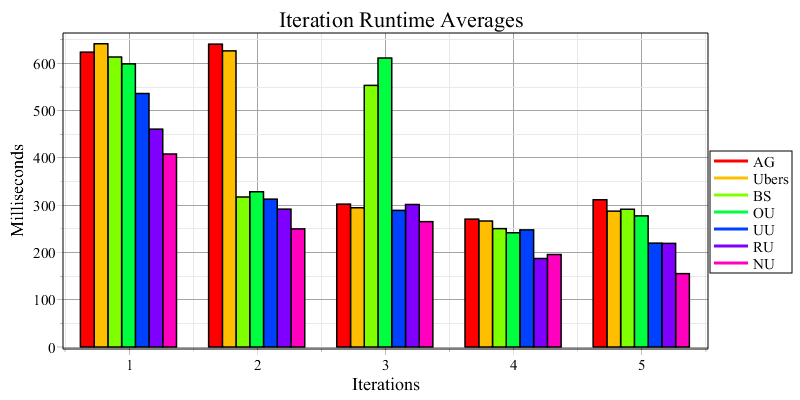
\includegraphics[width=0.9\textwidth]{RuntimeAverages.png}
	\centering
	\caption{}\label{RunTimeAveragesGraph}
\end{figure}
The data indicates some note-worthy phenomena:
\begin{enumerate}
	\item In general and per iteration, the more Pok\'emon that are allowed by a battle format, the longer it takes for SBPA to search for a solution. This was rather expected, since more data to process equates to a longer runtime. What is of interest is that there seems to be a linear correlation between the number of Pok\'emon that a format allows and the time required for SBPA to complete an iteration, as shown by Figure \ref{TierAmountGraph} in combination with Figure \ref{RunTimeAveragesGraph}. Whether this is a true linear correlation is hard to say: the possibility exists that there isn't enough data for the algorithm to start exhibiting non-linear characteristics. Only through the making of more formats can this hypothesis be tested.
	\item In general and per battle format, every iteration in the SBPA algorithm seems to take less time. This occurrence is again to be expected for much the same reasons as phenomena 1: every iteration processes less and less data by using the Species Clause and ignoring all Pok\'emon (and forms thereof) that have already been selected for the user's team. Phenomena 3 and 4, however, describe exceptions to this observation.
	\item During the second iteration for battle format BS (Battle Spot Singles) and OU (Overused), the SBPA algorithm requires around 325 milliseconds to run to completion. However, the iteration thereafter takes almost twice as long. This phenomena is odd, since it does not occur for any other format and defies all logic. Though unlikely, perhaps this occurrence results from faulty programming somewhere in the algorithm, but more research is needed to discover the exact origin of this phenomenon.
	\item During the second iteration, the algorithm requires around 300 milliseconds to run to completion for all but two battle formats. However, for the Anything Goes and Uber formats, SBPA still requires around 640 milliseconds. Both formats allow nearly identical sets of Pok\'emon species, which explains why the graphs for these two formats are so similar. However, it does not explain why the algorithm requires much less time to complete Iteration 2 for all other formats. More research is required to investigate this matter.
\end{enumerate}

\section{Conclusion}
The SBPA algorithm is an algorithm that gives advice on how to build a competitive Pok\'emon team. By analyzing the partial team the user already has, it uses simple mathematics to analyze Pok\'emon species on an individual level and determine the best potential team members based on Base Stats, Typing, and the Popularity Factor.\\\\
SBPA focuses on time efficiency and user interactivity. Through experimentation and algorithm runtime analysis, it has been shown that the algorithm can complete any iteration in less than a second, which is astronomically more time efficient than analyzing the over 200 trillion different Pok\'emon teams in order to find an optimum. Of course, different optimization techniques do exist that would find the optimal team in a time-efficient manner, but they would remove user-interactivity from the process. Therefore, albeit that SBPA is less accurate in determining the absolute optimum, the author finds that the algorithm's efficiency and user-friendliness is compensation enough.\\\\
The author does plan to continue developing SBPA into an even more accurate and time-efficient program. New scoring systems can be developed to give user's an even better understanding of the Pok\'emon they are working with. Optimization techniques can be implemented that allow users to be inspired by mathematically optimal teams. SBPA could be used as an app or website, made available for everyone. Hopefully one day, SBPA will be a huge aid for all trainers alike, united by one thing: Pok\'emon.

\newpage
\section{Acknowledgments and Bibliography}
\subsection{Acknowledgments}
Special thanks to Dr. K. P. Hart, Mathematician of General and Set-theoretic Topology at the Technical University of Delft, for his invaluable assistance as Bachelor Supervisor and Judge.\\\\
Also special thanks to the committee members Dr. Bart van den Dries and Dr. Dion Gijswijt, both Mathematicians at the Technical University of Delft.
\subsection{Bibliography}
\begin{enumerate}
	\item ``About the Pokémon Company International." Pok\'emon. The Pok\'emon Company International, n.d. Web. 15 June 2016. $<$http://www.pokemon.com/us/about-pokemon/$>$.
	\item ``Anything Goes." Smogon University, n.d. Web. 16 June 2016. \\$<$http://www.smogon.com/dex/xy/formats/ag/$>$. 
	\item ``Base stats." Bulbapedia, the Community-driven Pokémon Encyclopedia. Bulbagarden, n.d. Web. 16 June 2016. $<$http://bulbapedia.bulbagarden.net/wiki/Base\_stats$>$.
	\item ``Battle Spot Singles." Smogon University, n.d. Web. 16 June 2016. \\$<$http://www.smogon.com/dex/xy/formats/battle\_spot\_singles/$>$.
	\item ``Damage." Bulbapedia, the Community-driven Pokémon Encyclopedia. Bulbagarden, n.d. Web. 17 June 2016. $<$http://bulbapedia.bulbagarden.net/wiki/Damage\#Super\_effective$>$.
	\item ``Deoxys." Pok\'emon. The Pok\'emon Company International, n.d. Web. 15 June 2016. $<$http://www.pokemon.com/us/pokedex/deoxys$>$. 
	\item ``Gen VI Tiers." Smogon University, n.d. Web. 16 June 2016. \\$<$http://www.smogon.com/xyhub/tiers$>$. 
	\item Heijstek, Jenty.``Improvements to the SBPA Algorithm." Personal interview. 10 June 2016.
	\item``Introduction To Competitive Pok\'emon." Smogon University, 2013. Web. 15 June 2016. $<$http://www.smogon.com/dp/articles/intro\_comp\_pokemon$>$.
	\item ``List of Pokémon." Wikipedia. Wikimedia Foundation, n.d. Web. 16 June 2016. \\$<$https://en.wikipedia.org/wiki/List\_of\_Pok\%C3\%A9mon$>$.
	\item ``Making the Jump to Video Game Competitive Play." Pok\'emon. The Pok\'emon Company International, n.d. Web. 16 June 2016. \\$<$http://www.pokemon.com/us/strategy/making-the-jump-to-video-game-competitive-play/$>$.
	\item ``Neverused." Smogon University, n.d. Web. 16 June 2016. \\$<$http://www.smogon.com/dex/xy/formats/nu/$>$.
	\item ``Overused." Smogon University, n.d. Web. 16 June 2016. \\$<$http://www.smogon.com/dex/xy/formats/ou/$>$.
	\item ``Party." Bulbapedia, the Community-driven Pokémon Encyclopedia. Bulbagarden, n.d. Web. 16 June 2016. $<$http://bulbapedia.bulbagarden.net/wiki/Party$>$.
	\item ``Physical move." Bulbapedia, the Community-driven Pokémon Encyclopedia. Bulbagarden, n.d. Web. 17 June 2016. $<$http://bulbapedia.bulbagarden.net/wiki/Physical\_move$>$.
	\item ``Pokémon." Wikipedia. Wikimedia Foundation, n.d. Web. 15 June 2016. \\$<$https://en.wikipedia.org/wiki/Pok\%C3\%A9mon$>$. 
	\item ``Pokémon Battle." Bulbapedia, the Community-driven Pokémon Encyclopedia. Bulbagarden, n.d. Web. 16 June 2016. \\$<$http://bulbapedia.bulbagarden.net/wiki/Pok\%C3\%A9mon\_battle$>$.
	\item ``Pok\'emon File." Pok\'emon Showdown! Smogon University, n.d. Web. 17 June 2016. \\$<$http://play.pokemonshowdown.com/teambuilder$>$.
	\item ``Pokémon Types \& Type Chart." Pokémon Database, n.d. Web. 17 June 2016. $<$http://pokemondb.net/type$>$. 
	\item ``Pokémon VG World Championships." Pok\'emon. The Pok\'emon Company International, n.d. Web. 15 June 2016. $<$http://www.pokemon.com/us/play-pokemon/pokemon-events/pokemon-tournaments/vg-world-championships/$>$.
	\item ``Rarelyused." Smogon University, n.d. Web. 16 June 2016. \\$<$http://www.smogon.com/dex/xy/formats/ru/$>$.
	\item ``Special move." Bulbapedia, the Community-driven Pokémon Encyclopedia. Bulbagarden, n.d. Web. 16 June 2016. $<$http://bulbapedia.bulbagarden.net/wiki/Special\_move$>$.
	\item ``Statistic." Bulbapedia, the Community-driven Pokémon Encyclopedia. Bulbagarden, n.d. Web. 17 June 2016. $<$http://bulbapedia.bulbagarden.net/wiki/Statistic$>$.
	\item ``Type." Bulbapedia, the Community-driven Pokémon Encyclopedia. Bulbagarden, n.d. Web. 17 June 2016. $<$http://bulbapedia.bulbagarden.net/wiki/Type$>$.
	\item ``Uber." Smogon University, n.d. Web. 16 June 2016. \\$<$http://www.smogon.com/dex/xy/formats/uber/$>$.
	\item ``Underused." Smogon University, n.d. Web. 16 June 2016. \\$<$http://www.smogon.com/dex/xy/formats/uu/$>$.
	\item ``Zigzagoon." Pok\'emon. The Pok\'emon Company International, n.d. Web. 15 June 2016. $<$http://www.pokemon.com/us/pokedex/zigzagoon$>$.
\end{enumerate}
\section{Appendix}
For the actual code of the program, please visit the Github repository PokeTeam by HugoReijm:\\
\begin{center}
	https://github.com/HugoReijm/PokeTeam
\end{center}
\end{document}